\uuid{6986}
\auteur{blanc-centi}
\datecreate{2015-07-04}

\contenu{
\texte{
Montrer que la courbe paramétrée 
$$\left\{\begin{array}{l}x(t)=\frac{4t-3}{t^2+1}\\ \ \\ y(t)=\frac{2t-1}{t^2+2}\end{array}\right.$$
admet un unique point singulier, et tracer l'allure de la courbe au voisinage de ce point.
}
\indication{Un point $M(t)$ est singulier si $x'(t)=0$ et $y'(t)=0$.}
\reponse{
Les fonctions $x$ et $y$ sont de classe $\mathcal{C}^1$ sur $\R$. 
Un point $M(t)$ de la courbe est singulier si $x'(t)=y'(t)=0$, or
$$\left\{\begin{array}{l}
x'(t)=\frac{4(t^2+1)-2t(4t-3)}{(t^2+1)^2}=\frac{-2(2t^2-3t-2)}{(t^2+1)^2}\\
\ \\
y'(t)=\frac{2(t^2+2)-2t(2t-1)}{(t^2+2)^2}=\frac{-2(t^2-t-2)}{(t^2+2)^2}
\end{array}\right.$$
Ainsi $M(t)$ est singulier si et seulement si 
$\left\{\begin{array}{l}2t^2-3t-2=0\\t^2-t-2=0\end{array}\right.$. 
Ce système admet une unique solution $t=2$, correspondant au point $M(2)$ de coordonnées $(1,\frac{1}{2})$.

Le vecteur dérivé est nul au point $M(2)$ ; 
pour obtenir l'allure de la courbe au voisinage de ce point,
il faut donc effectuer un développement limité à un 
ordre assez grand pour trouver deux termes non constants non nuls. 
Ici l'ordre 3 suffira, on pose $t=2+h$ pour simplifier 
(ainsi ``$t$ proche de 2'' devient ``$h$ proche de 0''):
\begin{eqnarray*}
x(2+h)&=&\frac{4(2+h)-3}{(2+h)^2+1}=\frac{5+4h}{5+4h+h^2}=1-\frac{1}{5}h^2\cdot\frac{1}{1+\frac{4h+h^2}{5}}\\
 &=&1-\frac{1}{5}h^2\cdot\left(1-\left(\frac{4h+h^2}{5}\right)+o\left(\frac{4h+h^2}{5}\right)\right)\\
 &=&1-\frac{1}{5}h^2\cdot\left(1-\frac{4}{5}h+o(h)\right)\\
 &=&1-\frac{1}{5}h^2+\frac{4}{25}h^3+o(h^3)
\end{eqnarray*}
\begin{eqnarray*}
y(2+h)&=&\frac{2(2+h)-1}{(2+h)^2+2}=\frac{3+2h}{6+4h+h^2}=\frac{1}{2}-\frac{1}{12}h^2\cdot\frac{1}{1+\frac{4h+h^2}{6}}\\
 &=&\frac{1}{2}-\frac{1}{12}h^2\cdot\left(1-\left(\frac{4h+h^2}{6}\right)+o\left(\frac{4h+h^2}{6}\right)\right)\\
 &=&\frac{1}{2}-\frac{1}{12}h^2\cdot\left(1-\frac{2}{3}h+o(h)\right)\\
 &=&\frac{1}{2}-\frac{1}{12}h^2+\frac{1}{18}h^3+o(h^3)
\end{eqnarray*}
On a donc le développement limité vectoriel suivant:
$$M(2+h)=\begin{pmatrix}1\\ \frac{1}{2}\end{pmatrix}
+\begin{pmatrix}-\frac{1}{5}\\-\frac{1}{12}\end{pmatrix}\cdot h^2+
\begin{pmatrix}\frac{4}{25}\\  \frac{1}{18}\end{pmatrix}\cdot h^3+o(h^3)$$
On vérifie que le terme constant du développement limité correspond bien à 
$\begin{pmatrix}x(2)\\ y(2)\end{pmatrix}$ et que le terme linéaire, 
qui vaut $\begin{pmatrix}x'(2)\\ y'(2)\end{pmatrix}\cdot h$, est nul. 
Les coefficients de $h^2$ et $h^3$ sont des vecteurs non nuls, $M(2)$ 
est donc un point de rebroussement de première espèce ($p=2$, $q=3$).
La tangente est dirigée par le premier vecteur 
non nul, coefficient de $h^k$ (avec $k\ge1$), donc ici
le coefficient de $h^2$ ; ainsi la tangente en $M(2)$ est dirigée par 
$\left(\begin{smallmatrix}-\frac{1}{5}\\ -\frac{1}{12}\end{smallmatrix}\right)$.


\begin{center}
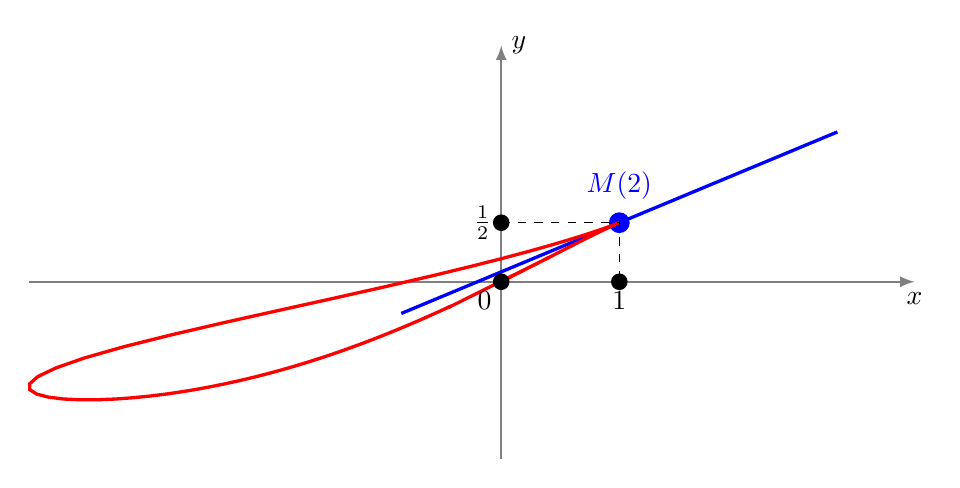
\begin{tikzpicture}[scale=1.5]
     \draw[->,>=latex,thick, gray] (-4,0)--(3.5,0) node[below,black] {$x$};
     \draw[->,>=latex,thick, gray] (0,-1.5)--(0,2) node[right,black] {$y$};  

  \coordinate (P) at (1,1/2);
  \fill[blue] (P) circle (2.5pt)  node[above=5pt]{$M(2)$}; 
  \draw[very thick, blue] (P)--+(22.6:2)--+(22.6:-2);

  \draw[red, very thick,domain=-10:10,samples=200] plot ({(4*\x-3)/(\x*\x+1)},{(2*\x-1)/(\x*\x+2)});

  \draw[red, very thick] (0,0)--+(27:0.45)--+(26:-0.5);


  \fill[black] (0,0) circle (2pt) node[below left]{$0$}; 
  \fill[black] (1,0) circle (2pt)  node[below]{$1$}; 
  \fill[black] (0,0.5) circle (2pt)  node[left]{$\frac12$}; 
  \draw[black, dashed] (0,0.5)--(1,0.5)--(1,0); 

\end{tikzpicture}  
\end{center}
}
}
